% Autor: Jose Ricardo Bustos Molina
%        Universidad del Tolima
%        jrbustosm@ut.edu.co
%

\section{Resultados y análisis}

Inicialmente se desarrollo la aplicación para teléfonos móviles de nombre CALINA, la cual permite en un 
entorno escolar tradicional usar gamificación bajo un contexto normal de clase presencial, esta aplicación 
se diseño bajo el precepto de ser un apoyo al desarrollo de la clase sin robar mucho protagonismo o tiempo al 
docente o los estudiantes.  Por otro lado, se construyo la aplicación para que no tenga la necesidad de usar 
el servicio de datos ni una conexión a Internet por motivo del contexto local en el cual no es normal contar 
con cobertura o la vinculación a este servicio.

\begin{figure}[!htb]
\caption[Aplicación CALINA, pantalla principal]{Aplicación CALINA, pantalla principal}
\centering
\begin{adjustbox}{width=6cm}
\begin{tikzpicture}
	\node[inner sep=0pt] at (0cm,0cm) {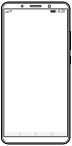
\includegraphics[width=7cm]{screenshots/movil}};
	\node[inner sep=0pt] at (-0.05cm,0.05cm) {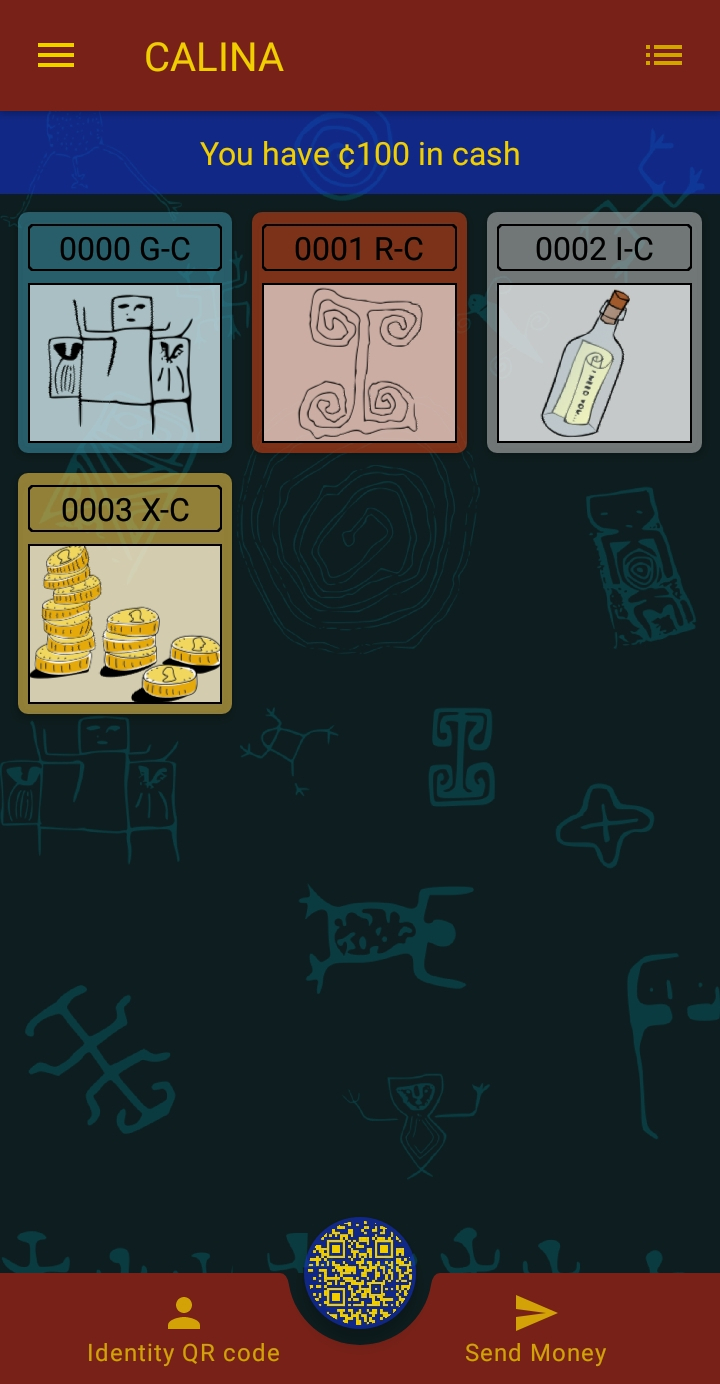
\includegraphics[width=5.95cm]{screenshots/pantalla_principal}};
\end{tikzpicture}
\end{adjustbox}
\\
{\footnotesize Fuente: de elaboración propia}
\end{figure}

Para el diseño de esta aplicación, se decidió darle importancia especial al uso de diégesis, incluso en la 
misma interfaz de la aplicación, por lo que se selecciono colores de uso locales e iconografía de los pueblos 
originarios, incluso el nombre de la aplicación es extraída del contexto local. Esto con el fin de darle una 
capa de narración adicional al software en sí.

Paralelo a esto se aplico la primera encuesta no estructurada para conocer algunos requerimientos y 
perspectivas del docente que va a aplicar la estrategia gamificada CALINA, esta encuesta se puede leer en el 
anexo \label{anexo:encuestas}, de ella podemos extraer algunos párrafos.

\makeatletter
\newcommand*{\singlespacingNoVspace}{%
  \setstretch{\setspace@singlespace}}
\makeatother

\newenvironment{singlequote}
  {\quote\small\singlespacingNoVspace}
  {\endquote}

\SetBlockEnvironment{singlequote}

\begin{displayquote}
	\dots quería saber que sabes sobre gamificación, lo has usado en tus clases?

	\dots referido a utilizar juegos en el aula o ambiente de aprendizaje \dots suelo usar juegos de 
	memoria, vídeo lecciones, juegos de mesa (bingo, serpiente)

	\dots aprender mediante actividades lúdicas \dots para que le sea mas fácil su comprensión
\end{displayquote}

Podemos inferir que la docente al inicio de la entrevista no diferencia bien los conceptos de gamificación y 
ludificación, el cual es un error común entre los docentes, era necesario aclarar esto para la buena 
aplicación de la estrategia ya que no se piensa desarrollar un juego, si no una estrategia que complementa el 
desarrollo normal de la clase que va a impartir. Por otro lado, el docente manifiesta una relevancia por el 
uso de actividades lúdicas para que la comprensión de los temas sea más fácil.

\begin{displayquote}
	\dots estrategia sencilla como poner un sello \dots

	\dots se vuelve un incentivo por su participación en clase no por un buen comportamiento, que puede al 
	final del periodo contribuir a mejorar la nota final

	Incentivan a culminar las actividades, a participar aunque se equivoquen ya que no solo lo reciben el 
	sello por que este bien la respuesta. Muchos buscan de cierta manera recibir su sello; algunos lo 
	hacen porque requieren al final de corte subir su promedio, otros por validar que su trabajo este
	bien y que hayan comprendido
\end{displayquote}

La docente suele usar sellos como incentivos en las notas de sus estudiantes y para motivar su participación, 
es consiente de que su estrategia incrementa la participación, mas no los usa como un reforzamiento 
conductual ni deforma positiva ni negativa. Usando la estrategia de sellos manifiesta que hay dos razones que 
motivan a sus estudiantes a buscar obtenerlos: Aumento de nota y reconocimiento de su aprendizaje.

\begin{displayquote}
	\dots En otros contextos, ahora que los jóvenes se preparan para el \textit{English day}, los uso para 
	seleccionar los competidores de un concurso de deletreo \dots
\end{displayquote}

La docente manifiesta que usa el concurso de deletreo en su colegio para motivar en los estudiantes 
sobresalientes un reto para su progreso en los temas de la asignatura, y usa incentivos con ellos para que se 
vinculen y participen en la actividad voluntaria.

\begin{displayquote}
	Busco actividades con canciones en Inglés, canciones con algún artista que les guste y este acorde al 
	tema a trabajar, vídeo lecciones con personajes animados o de películas que les gusten para fortalecer 
	la escritura o vocabulario.
\end{displayquote}

En el desarrollo de su guía de aprendizaje la docente involucra narrativas diferentes a las del tema del 
curso, para esto involucra motivación intrínseca en los estudiantes usando sus propios gustos, como pueden ser 
vídeo juegos que suelen usar, canciones, películas, o artistas, con tal de interesar a los estudiantes e 
incluso usar un vocabulario que todos ya suelan manejar.

\begin{displayquote}
	\dots realiza de antemano una planificación de los incentivos y puntos extras \dots

	Va surgiendo en el desarrollo de la clase
\end{displayquote}

La planificación de los incentivos no es planeada por la docente, su creación, significado y reglas van 
surgiendo a medida del desarrollo de su ejercicio docente.

\begin{displayquote}
	\dots un espacio para aprender ya que el miedo de ellos es muchas veces hablar y pronunciar \dots 

	\dots en lo social-relacional que interactúe con sus compañeros \dots

	\dots que no sean atractivos para el estudiante al punto en que no participen o no les ayude a 
	aprender, que este (os) no los aproveche y se pierda el objetivo de la clase \dots
\end{displayquote}

Respecto a los sentimientos o dinámicas que puede mencionar la docente se encuentra el miedo a participar en 
clase, el cual incrementar esta participación se hace muy importante por tratarse de un curso del idioma 
inglés, lo cual tiene mucho que ver con la dinámicas que surgen de su interacción con el docente y compañeros. 
Por otro lado manifiesta un miedo interno en cuanto a la no utilización o compresión de los puntos extras o
incluso la perdida de perspectiva de su clase al incluir un elemento adicional.

Posterior a esto se aplicó la estrategia gamificada y usando juegos de Rol a los grupos G\textsubscript{2} y 
G\textsubscript{3} respectivamente, dejando al grupo G\textsubscript{1} sin el uso de gamificación para tener 
una perspectiva sin dicha implementación. Estrategias que se aplicaron en las clases de solo una semana, con 
los estudiantes que desearon usarla por voluntad propia y que tenían los equipos móviles aptos para la 
ejecución de la aplicación CALINA desarrollada.

A continuación se aplicó la entrevista no estructurada final la cual se puede ver en el anexo 
\label{anexo:encuestas}, de esta entrevista extraigo y se da una interpretación de lo dicho por la docente.

\begin{displayquote}
	\dots se requiere un trabajo extra pero en cuanto a planear como se va a hacer uso de la estrategia en 
	clase, por supuesto facilita el proceso en cuanto a que puede lograr que el estudiante se motive a 
	participar \dots
\end{displayquote}

Se puede evidenciar que la docente al desarrollar la guía pedagógica se hizo un trabajo conjunto para la 
planificación de la estrategia gamificada usando el modelo de capas propuesto, lo que requiere un trabajo 
adicional para el docente, sin embargo, manifiesta un beneficio al usar la estrategia con los estudiantes en 
clase haciendo más ágil, asequible y atractivo el proceso de adjudicación de puntos extras.

\begin{displayquote}
	\dots esta estrategia si considero motiva al estudiante \dots

	\dots Podría desmotivar si el estudiante cree que no tiene o no puede hacer parte de las actividades u 
	obtener incentivos por no contar con la app \dots

	\dots para ellos es mas emocionante intercambiar cartas, obtener medallas, dragones etc, que un sello 
	en un cuaderno\dots
\end{displayquote}

La estrategia CALINA según la docente reporta resultados positivos respecto a la motivación de los estudiantes 
que usaron la aplicación, sin embargo, manifiesta preocupación por los estudiantes que no pudieron usar la 
aplicación por no poseer móvil o que no pudieron ganar puntos de experiencia, respecto al último puntos, es 
bueno mejorar el plan pedagógico creado, para así incluir reglas que aumenten la opción de ganar puntos de 
experiencia y cartas de acción para motivar su participación.

\begin{displayquote}
	\textbf{Reconocimiento} al sentir que sus compañeros lo reconocen por sus habilidades. 
	\textbf{Socialización} al interactuar dentro de las actividades propuestas para lograr que se cumpla 
	la estrategia o se obtengan los incentivos.

	\textbf{Fantasía}, ya que la misma estrategia propone historias para recibir cartas con determinados 
	personajes. Esto lleva a que el estudiante se involucre.
\end{displayquote}

La docente da ejemplos de como mediante el uso de la estrategia planteada se generan en los estudiantes 
sentimientos que mediante el uso de una estrategia normal no se manifiestan o se manifiestan en menor medida, 
la evocación de dichos sentimientos tiene como objetivo motivar e inspirar al estudiante en el desarrollo de 
su proceso de aprendizaje.

\begin{displayquote}
	\dots Mejora el rendimiento escolar ya que entre más participación del estudiante \dots hay una mayor
	comprensión de los temas o competencias tratadas en clase \dots

	\dots En cuanto a disposición, como son jóvenes si varía dependiendo a veces del estado de ánimo de 
	ellos \dots
\end{displayquote}

En cuanto al aumento del rendimiento escolar la docente indica que mejora el rendimiento escolar debido a un 
incremento en la participación de los estudiantes, y existe una mejoría en la comprensión de los temas debido 
a este incremento de la participación. Por otro lado, la docente manifiesta que esto no se aplica en 
estudiantes que a priori vengan con un estado de animo bajo.

\begin{displayquote}
	Ambas funcionan bien, en la primera algunos indagaron sobre el significado de los símbolos y de las 
	cartas, en la segunda la historia les causó curiosidad por saber de dónde surgió la historia y los 
	hizo fantasear o sentirse parte de ella y a otros diversión.
\end{displayquote}

Respecto al uso de estrategia gamificada y la estrategia usando narrativas, la docente manifiesta que las dos 
estrategias funcionan, indicando que en la primera genero sentimientos de exploración y la segunda inspiró
sentimientos de fantasía y curiosidad.

\begin{displayquote}
	El tiempo para su aplicación en clase a sido corto por lo que entre los grupos no he identificado 
	alguna interacción que involucre la estrategia sin embargo dentro de la clase si entre los jóvenes, 
	están hablando de la estrategias, miran con curiosidad y exploran la aplicación y que se puede hacer
	con ella lo que ha llevado a que socialicen aun más entre ellos.
\end{displayquote}

La docente no pudo observar dinámicas surgidas entre los tres grupos, sin embargo, si aprecia dinámicas 
surgidas entre los estudiantes del mismo curso, logrando dinámicas sociales de cooperación e indagación, 
manifiesta que esto puede ser debido al corto tiempo de la prueba.

\begin{displayquote}
	Aspectos positivos: la aplicación tiene un diseño muy hermoso, los colores son muy del Tolima y para 
	los estudiantes es muy intuitivo, fácil de entender y usar. 
\end{displayquote}

En cuanto a los aspectos positivos a resaltar, dice la docente que la aplicación tienen una interfaz gráfica 
agradable e intuitiva, y muestra agrado por el tema local de la aplicación.

\begin{displayquote}
	En cuanto a mejorar, se requiere mejorar o hacer más fácil aún la manera de crear las cartas ya que la 
	opción de opciones avanzadas ``\textit{trigger}'' requiere ser un poco más especializado para crear una carta 
	con cosas especiales. Se trata entonces de que el docente deba leer mejor el manual para poder 
	optimizar el uso de la app en clase quizás es algo que no todos vayan a hacer y por lo tanto pueden 
	desechar su uso.
\end{displayquote}

Finalmente en cuanto a características a mejorar, manifiesta que el uso de los ``\textit{triggers}'' puede 
llegar a ser complejo y confuso.
